\documentclass{SGGW-thesis}
\graphicspath{ {./images/} }

\INZYNIERSKAtrue
\WZIMtrue

\listfiles

\title{Porównanie aplikacji frontendowych opartych na mikrofrontendach z tradycyjną architekturą monolityczną na przykładzie aplikacji do zarządzania finansami osobistymi}
\Etitle{Comparison of Microfrontend Applications and Monolith Frontend Applications Based on the Example of Expense Tracker}
\author{Dawid Wijata}
\date{2023}
\album{205006}
\thesis{Praca dyplomowa na kierunku:}
\course{Informatyka}
\promotor{dr. \ inż.\ Piotra Wrzeciono}
\pworkplace{Instytut Informatyki Technicznej\\Katedra Systemów Informacyjnych}

\raggedbottom

\begin{document}
\counterwithout{figure}{chapter}
\counterwithout{lstlisting}{chapter}

\maketitle
\statementpage
\abstractpage
{Porównanie aplikacji frontendowych opartych na mikrofrontendach z tradycyjną architekturą monolityczną na przykładzie aplikacji do zarządzania finansami osobistymi}
{Tematem niniejszej pracy była implementacja i poźniejsze porównanie frontendu dwóch wersji aplikacji do zarządzania finanasami osobistymi w dwóch architekturach - mikrofrontendowej i monolitycznej. Praca składa się z części teoretycznej wprowadzającej w pojęcie mikroserwisów i mikrofrontendów oraz części praktycznej porównującej obie implementacje pod względem metryk kodu, wydajności, kosztów obu rozwiązań oraz zarządzania projektem.}
{architektura rozproszona, mikroserwisy, mikrofrontendy, architektura oprogramowania}
{Comparison of Microfrontend Applications and Monolith Frontend Applications Based on the Example of Expense Tracker}
{The subject of this thesis was to implement and compare frontend parts of expense tracker web application written in two different architectural concepts - monolith and microfrontends. The first part is an introduction to microservice and microfrontend concepts. The second one consists of a comparison of both application versions by terms of code metrics, performance, financial costs of both solutions and project management.}
{distributed architecture, microservices, microfrontends, software architecture}



% Spis treści może być złożony z pojedynczą interlinią, np. jeśli jedna linia wychodzi na następną stronę.
% W przeciwnym razie spis treści wstawić bez powyższego rozkazu i klamry.
{
	\doublespacing
	\tableofcontents
}

\startchapterfromoddpage % niezależnie od długości spisu treści pierwszy rozdział zacznie się na nieparzystej stronie

\chapter{Wprowadzenie do mikroserwisów}
% tu wstęp
\section{Architektura monolityczna}
Monolitem, bądź programem zaprojektowanym zgodnie z architekturą monolityczną nazywamy program uruchamiany w całości za pomocą jednego pliku wykonywalnego. W~aplikacjach webowych taka architektura spełnia założenia modelu trójwarstwowego. Na te warstwy składają się:

\begin{enumerate}
	\item interfejs użytkownika składający się z dokumentów HTML, arkuszy styli CSS oraz skryptów JavaScript definiujących zachowanie interfejsu użytkownika,
	\item warstwa API przygotowująca dane podawane do interfejsu użytkownika w celu pokazania go użytkownikowi,
	\item warstwa dostępu do danych.
\end{enumerate}

Taką strukturę trójwarstwową możemy opisać diagramem z \cref{fig:monolith_diagram}

\begin{figure}[h]
	\centering
	\captionsetup{justification=centering}
	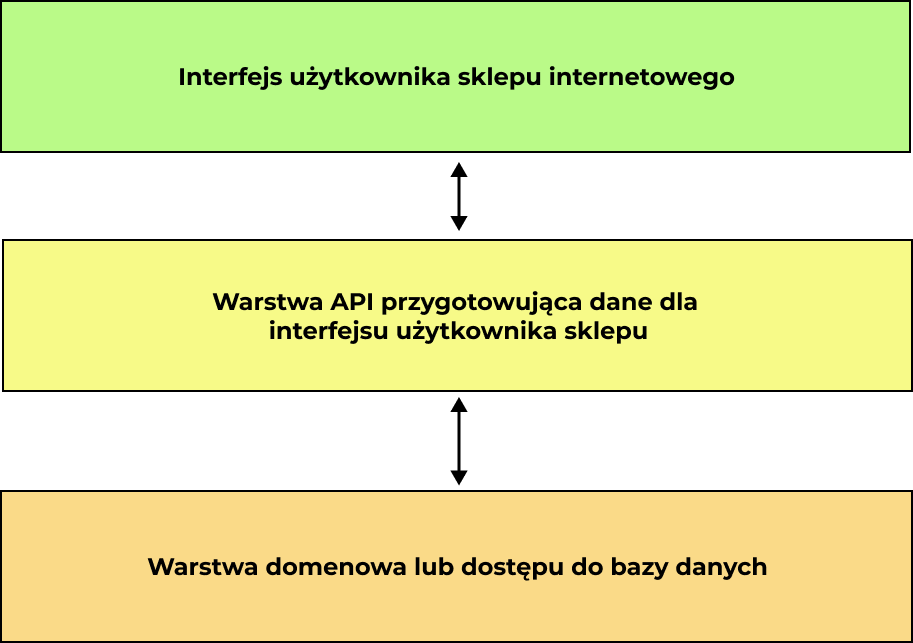
\includegraphics[width=0.8\textwidth]{monolith_diagram.png}
	\caption{Podział na warstwy dla przykładowego sklepu internetowego \\ w architekturze monolitycznej}
	\label{fig:monolith_diagram}
\end{figure}

Warstwa druga jest czasami pomijana przez twórców oprogramowania pozwalając interfejsowi użytkownika na bezpośredni dostęp do danych. Różnicą między nimi jest brak istnienia warstwy oddzielającej logikę biznesową od interfejsu użytkownika. Wtedy możemy mówić o modelu dwuwarstwowym.
Wraz z rozwojem aplikacji w modelu dwuwarstwowym i trójwarstwowym oraz ciągłemu dopisywaniu do nich nowych funkcjonalności, kod tych aplikacji stawał się coraz bardziej nieczytelny, a zależności między fragmentami kodu okazywały się być zbyt rozwlekłe.
Ponadto każda zmiana w~oprogramowaniu powoduje konieczność zbudowania oraz wystawienia na środowisko produkcyjne kolejnej wersji oprogramowania. Przy dużych aplikacjach ten proces potrafi zabierać znaczącą ilość czasu. Utrudnia to też proces testowania oprogramowania, zarówno manualnie (ze względu na rosnącą ilość scenariuszy testowych) jak i automatycznie (ze względu na rosnący czas uruchomienia siatki testów).
Zgodnie z prawem Conway'a, takie trudności odbijają się na sposobie zarządzania organizacją, która jest producentem oprogramowania.
Zgodnie z \cite{fowler}, pojęcia \textit{monolit} w odniesieniu do oprogramowania pierwotnie używała społeczność programistów systemu operacyjnego Unix. Programiści Unix'a określali tak systemy, które stają się zbyt duże, by móc je komfortowo utrzymywać.

\section{Architektura mikroserwisów}

Trudności z utrzymaniem oprogramowania, które w obrębie jednego projektu zawiera ciągle rozrastającą się logikę, spowodowały konieczność zastosowania podziału kodu na mniejsze i jednocześnie prostsze w utrzymaniu części.
W związku z tym do większych aplikacji zaczęto stosować ich podział na części będące usługami niezależnymi od pozostałych elementów systemu. Taką pojedynczą usługę nazywamy mikroserwisem. Przykładowe rozmieszczenie modułów w projekcie mikroserwisowym możemy zaobserwować na \cref{fig:microservices_diagram}

\vfill
\clearpage
% ogarnąć tekst tak, aby rysunek wyświetlał się w poprawnym miejscu

\begin{figure}[h]
	\centering
	\captionsetup{justification=centering}
	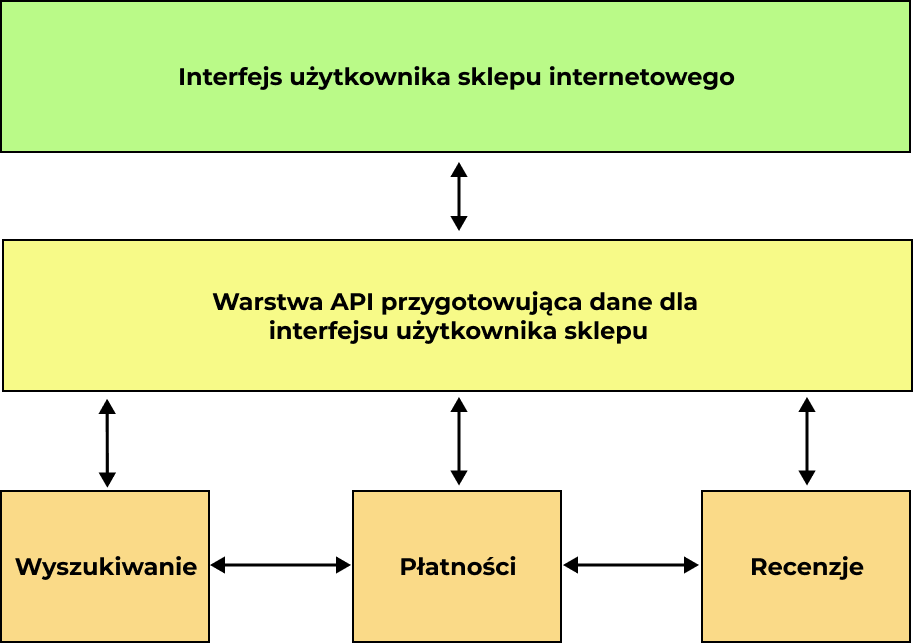
\includegraphics[width=0.8\textwidth]{microservices_diagram.png}
	\caption{Podział na moduły dla przykładowego sklepu internetowego \\ w architekturze mikroserwisowej}
	\label{fig:microservices_diagram}
\end{figure}


Komunikacja między mikroserwisami zachodzi przy użyciu protokołów sieciowych neutralnych w ujęciu technologicznym, na przykład HTTP. Podział aplikacji na serwisy pozwala na wykonywanie prac nad konkretnymi funkcjonalnościami aplikacji bez potencjalnego ryzyka naruszenia kodu odpowiedzialnego za inne funkcjonalności. Innymi zaletami tego rozwiązania są:

\begin{enumerate}
	\item dowolność w zastosowaniu technologii - pozwala na użycie do każdej funkcjonalności zasobów technologicznych najlepiej odpowiadających danemu zadaniu,
	\item stabilność - ewentualne problemy z aplikacją nie powodują zatrzymania całego systemu, a jedynie konkretnego serwisu,
	\item skalowalność - nowe funkcjonalności można dodawać poprzez dodanie nowych serwisów, a poszczególne serwisy można rozszerzać nie naruszając logiki innych serwisów,
	\item wzrost dostępności usług - w razie, gdyby któryś z serwisów przestał działać, inne usługi nadal będą dostępne.
\end{enumerate}

Przedstawione zalety są znaczące nie tylko z punktu widzenia projektowania i tworzenia oprogramowania, ale też z punktu zarządzania projektami. Jasny podział projektu na niezależne od siebie części pozwala też na przyporządkowanie ludzi do zespołów mniejszych, ale ściśle skoncentrowanych na konkretnym wycinku wiedzy potrzebnym do realizacji danej funkcjonalności.
Autonomiczność takich zespołów pozwala na zmniejszenie ilości potrzebnych kontaktów między zespołami w celu ustalenia rozwiązań problemów i dalszego przebiegu projektu. Pomaga to między innymi zmniejszyć ilość spotkań oraz skrócić te krytycznie potrzebne do realizacji projektu.

Pomimo wielu zalet, architektura mikroserwisowa nie jest wolna od wad. Pierwszą z~nich są koszty infrastruktury potrzebnej do wdrożenia oprogramowania opartego na mikroserwisach. Aby spełnić postulat niezależności mikroserwisów od siebie, każdy oddzielny mikroserwis musi być postawiony na osobnym serwerze. W wyniku tego, zamiast zapłacić koszty utrzymania jednego serwera z lepszymi parametrami, zmuszeni jesteśmy zreplikować poniesione koszty na każdy z istniejących mikroserwisów.

Rozrośnięcie się infrastruktury przy użyciu mikroserwisów zwiększa też zapotrzebowanie na ludzi zajmujących się wsparciem developerów w zakresie konfiguracji infrastruktury (tzw. \textit{inżynierowie DevOps}), a w przypadku zastosowania technologii chmurowych, również specjalistów w zakresie technologii takich jak \textit{Microsoft Azure}, \textit{Google Cloud} oraz \textit{Amazon Web Services}. Taka sytuacja również przyczynia się do zwiększenia kosztów związanych z oprogramowaniem w architekturze mikroserwisowej. Można jednak uznać ją za czynnik zmuszający firmy do rozwoju w~zakresie R\&D (\textit{Research and Development}) w celu ustalenia własnych standardów architektonicznych, które będą optymalne dla ich potrzeb biznesowych w zakresie realizacji mikroserwisów. Mimo to, czynniki kosztowe powodują, że wybór architektury mikroserwisowej do projektu może nie być optymalny dla małych i średnich projektów.

Mikroserwisy powodują też konieczność uzgodnienia konwencji między projektami w~sprawach takich jak:

\begin{itemize}
	\item postać wyjątków rzucanych przez serwisy,
	\item opis obiektów, które są częścią innych serwisów,
	\item sposób łączenia się między serwisami,
	\item autoryzacja i uwierzytelnianie,
	\item standard podziału kodu na projekty lub moduły.
\end{itemize}
Brak zgody między projektami w powyższych kwestiach może doprowadzić do jeszcze większego nieporządku, niż gdyby projekt był realizowany jako monolit. Ponadto, uporządkowana struktura projektu mikroserwisowego pozwala na replikowanie schematu na dowolną skalę, a co za tym idzie, automatyzację procesu tworzenia nowych serwisów. Można to zrealizować na przykład za pomocą szablonów projektu aplikowanych do środowiska programistycznego, obrazów środowiska \textit{Docker} lub idąc jeszcze dalej - odpowiednio ustawionym klastrze \textit{Kubernetes}. Jednak przy sprostaniu tym wyzwaniom architektonicznym na etapie projektowania oprogramowania zyskamy dzięki mikroserwisom możliwość zarządzania projektem o dowolnej wielkości w sposób ściśle uporządkowany i z zachowaniem dobrej jakości kodu źródłowego oraz łatwe dostosowanie projektu do potrzeb biznesowych i metodologii zwinnych zarządzania projektami.

\chapter{Mikrofrontendy}
\section{Wstęp}
Pomimo zastosowania mikroserwisów przy projektowaniu logiki backendowej części aplikacji, frontendowa część projektu pozostawała w przeszłości mniej rozbudowana. Głównym powodem był fakt, że logika obliczeniowa i biznesowa występowała po stronie backendu. Odciążało to część frontendową, co pozwalało na mniejsze jej rozbudowanie oraz ograniczenie rozwarstwienia frontendu w postaci monolitu. Jednak wraz z rozwojem technologicznym w zakresie webowych interfejsów użytkownika, objętość kodu frontendowego w widoczny sposób wzrosła. Na taki stan rzeczy złożyło się wiele czynników takich jak:

\begin{itemize}
	\item powstawanie coraz bardziej kreatywnych i szczegółowych efektów wizualnych,
	\item optymalizacja działania skryptów JavaScript,
	\item zwiększająca się dojrzałość działalności programistów frontendu,
	\item rozwój frameworków strukturyzujących projekty frontendowe takich jak \textit{Angular}, \textit{React}, \textit{Vue} (produkują one dziesiątki tysięcy linii kodu wynikowego).
\end{itemize}

Wszystkie te czynniki spowodowały potrzebę podzielenia kodu na pewnego rodzaju moduły. Najpopularniejsze frameworki radzą sobie jednak wystarczająco dobrze ze skutkami nagromadzenia dużej ilości kodu, aby używać ich w projektach komercyjnych. Najlepiej z tym problemem radzi sobie framework Angular, który proponuje programistom systemowy podział na moduły, oraz kilka propozycji na podziały niższego stopnia na struktury takie jak:

\begin{itemize}
	\item component,
	\item service,
	\item guard,
	\item pipe
	\item i inne, rzadziej używane.
\end{itemize}

Jednak struktura organizacyjna całego projektu oprogramowania różni się znacząco po stronie backendu, jak i frontendu. Może to powodować różne nieścisłości organizacyjne oraz zwiększać liczbę zapytań wykonanych między członkami zespołu w celu uzgodnienia szczegółów projektu. Zaczęto się więc rozglądać za sposobem organizacji pracy zespołu frontendowego takiego, żeby móc podzielić osoby pracujące nad projektem na zespoły w pełni skoncentrowane na konkretnych funkcjonalnościach. Takie podejście zwiększa autonomiczność zepsołów.
Takim sposobem okazało się być dostosowanie frontendowych części projektu do architektury mikroserwisowej. Zgodnie z rysunkiem \cref{fig:microfrontends_diagram} można podzielić zespół programistów frontendu na funkcjonalne grupy dostosowane do wcześniej utworzonych podzespołów tak, aby wynikowe podzespoły były już w pełni skoncentrowane na wydzielonej partii wartości biznesowej.

\begin{figure}[h]
	\centering
	\captionsetup{justification=centering}
	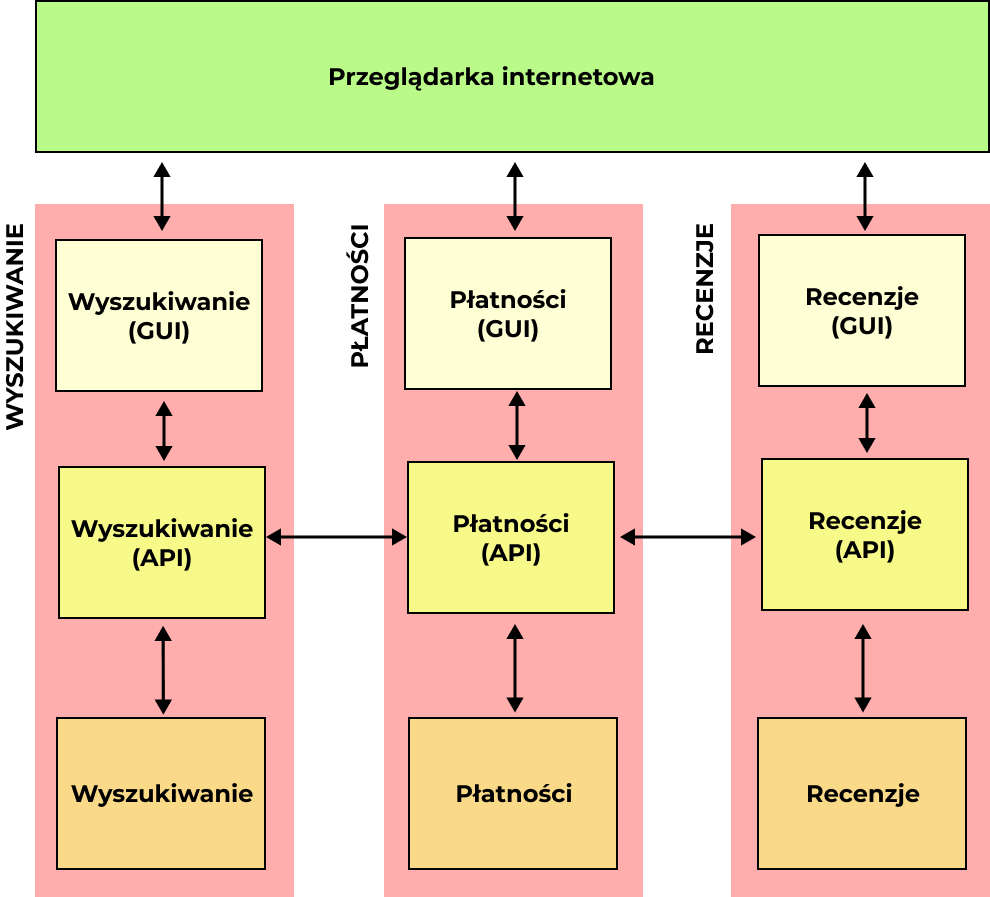
\includegraphics[width=0.8\textwidth]{microfrontends_diagram.png}
	\caption{Podział na moduły dla przykładowego sklepu internetowego \\ w architekturze mikrofrontendowej}
	\label{fig:microfrontends_diagram}
\end{figure}

Pojedynczą jednostkę funkcjonalną takiego podziału na frontendzie nazywamy \textit{mikrofrontendem}, a w ogólności architekturę używającą takiego podziału nazywamy architekturą mikrofrontendową.
Zgodnie z wynikami ankiety \cite{tsh_2022}, 24.6\% programistów biorących udział w ankiecie pracowało w 2021 roku w zespołach wykorzystujących w~projekcie architekturę mikrofrontendową. Ponadto, według tej ankiety, 37.2\% programistów biorących udział w ankiecie twierdzi, że w przeciągu dwóch następnych lat popularność koncepcji mikrofrontendów wzrośnie. Na podstawie tych statystyk można wnioskować, że pomysł rozszerzenia mikroserwisów na część frontendową przyjął się w~dużej części organizacji oraz przede wszystkim, w świadomości programistów.

\section{Dodatkowe ograniczenia względem mikroserwisów}
\subsection{Ograniczone zasoby obliczeniowe}
W przypadku prac nad backendowymi częściami projektu, coraz mniej zwraca się uwagę na optymalizację działania algorytmów używanych w oprogramowaniu. Pamięć operacyjna oraz masowa stały się dużo tańsze niż kilka lat temu. Dla klienta stało się tańsze zainwestowanie maksymalnie kilku tysięcy złotych na dołożenie pamięci do serwera, udostępniającego żądaną usługę sieciową, niż zainwestowanie wielokrotności tej kwoty w~czas pracy programistów, którzy zoptymalizują wadliwy algorytmicznie kod.
Nie ma to jednak zastosowania przy pracy nad frontendem. Przeglądarka, w której koniec końców efekty pracy są pokazane użytkownikowi końcowemu, oferuje jedynie swoje zasoby pamięci - nie można użyć tak dużego odsetka zasobów komputera, jak w przypadku backendu. Poza tym, minimalne odstępstwa od optymalizacji są zauważalne dla użytkownika końcowego. Każde przycięcie się elementów interfejsu, brak płynności powodują irytację użytkownika, a co dalej za tym idzie, spadek zadowolenia z używania wyprodukowanego oprogramowania. W przypadku zastosowania mikrofrontendów problem narasta. De facto ładujemy do przeglądarki jednocześnie kilka pełnoprawnych aplikacji i wymagamy od nich, aby one wszystkie podzieliły się niewielkimi zasobami pamięci i procesora zaalokowanymi przez przeglądarkę w taki sposób, aby każda z nich działała w sposób komfortowy dla użytkownika. Na szczęście rozwiązanie problemu jest konceptualnie bardzo proste. Wystarczy ładować do przeglądarki tylko te mikrofrontendy, które w danym momencie są użytkownikowi krytycznie potrzebne. Najczęściej stosowanym sposobem implementacji takiego rozwiązania jest ładowanie konkretnych mikrofrontendów po zmianie adresu URL w przeglądarce. Gotowe rozwiązania implementujące mikrofrontendy, takie jak \textit{Single SPA} optymalizują ładowanie zasobów jeszcze bardziej poprzez zastosowanie wzorca \textit{Lazy loading}. Dzięki tej prostej sztuczce, można ściśle kontrolować ładowanie się mikrofrontendów do przeglądarki.

\subsection{Zasoby współdzielone}
W przypadku, gdy na potrzeby jednego z mikrofrontendów tworzony jest reużywalny komponent (przykładowo tabela o odpowiednim wyglądzie i zachowaniu), może zaistnieć potrzeba zastosowania takiego komponentu w innym mikrofrontendzie. Wtedy pierwszym z pomysłów, jakie mogą powstać, jest przekopiowanie kodu z jednego do drugiego mikrofrontendu. Jednak to rozwiązanie tworzy nowe problemy.

Po pierwsze, każda zmiana w komponencie, w celu uzgodnienia wersji wymaga zmian w tym samym komponencie we wszystkich mikrofrontendach używających tego projektu. W przypadku kilku mikrofrontendów jest to możliwe, ale w przypadku, gdy mamy takich mikrofrontendów setki lub tysiące, takie cykliczne zmiany są wręcz niemożliwe do wykonania i zabierałyby one duży odsetek czasu poświęconego na projekt.
Rozwiązaniem problemu okazuje się być umieszczeniu tego kodu jedynie jeden raz w zewnętrznym repozytorium (technicznie mogą to być prywatne repozytoria NPM lub inne rozwiązanie) i~zainstalowanie przez użycie systemu zarządzania pakietami. We frontendowych częściach projektu najczęściej są to NPM i Yarn.

Po drugie, komponent skopiowany wprost z jednego mikrofrontendu na drugi, powoduje konieczność powstawania oddzielnych scenariuszy testowych na ten sam komponent dla każdego mikrofrontendu. W praktyce, już przy kilkunastu mikrofrontendach taka ilość testów staje się nie do utrzymania w takim stanie, aby scenariusze odpowiadały aktualnemu stanowi funkcjonalności.

\subsection{Arkusze styli CSS}
Arkusze styli z poszczególnych mikrofrontendów są ładowane razem do przeglądarki, na której uruchomiony jest każdy z pożądanych mikrofrontendów. Występuje w takiej sytuacji ryzyko replikacji tych samych styli CSS oraz nadpisywania się styli CSS między mikrofrontendami. Drugi z przypadków jest szczególnie kłopotliwy, gdyż wygląd niektórych elementów na stronie może zależeć wyłącznie od tego, który z mikrofrontendów załaduje się do przeglądarki jako pierwszy. Jest na to kilka rozwiązań:

\begin{itemize}
	\item stosowanie ogólnej konwencji nazewniczych dla klas CSS, takich jak BEM i OOCSS,
	\item wstrzykiwanie styli CSS bezpośrednio przez kod JavaScript (tzw. CSS-in-JS),
	\item zastosowanie Shadow DOM.
\end{itemize}

Każde z tych podejść wciąż wymaga dyskusji między programistami pracującymi nad projektem oraz ich ostrożności i uważności na aspekt nadpisywania się bądź replikacji styli CSS. Dlatego też, mimo opisanych ścieżek rozwiązania, najważniejsze stają się zdrowy rozsądek osób decydujących o przebiegu projektu oraz doświadczenie zespołu pracującego nad projektem.

\subsection{Komunikacja między mikrofrontendami}
W projektach zdarzają się sytuacje, gdy istnieje potrzeba ukazania na widoku frontendu informacji z kilku wycinków domenowych projektu. Dla sytuacji z  \cref{fig:microfrontends_diagram}, zaistniałoby to wtedy, gdyby do listy recenzji należało dodać informację, ile recenzujący użytkownik kupił sztuk produktu oraz za jaką kwotę. Określając to modułami z tego przykładu - do modułu mikrofrontendu realizującego recenzje produktów należałoby dodać komunikację z~mikrofrontendem obsługującym płatności. Rekomendowanym  zachowaniem w tej sytuacji jest nie stosować komunikacji między aplikacjami na frontendzie. Odrobinę lepszym wyjściem jest zastosować taką komunikację po stronie backendu i na warstwie API aplikacji stworzyć endpoint, który podaje do frontendu potrzebne informacje. Martin Fowler w swoim artykule \cite{fowler_2019} wspomina, że możliwe jest tutaj zastosowanie wzorca architektonicznego BFF (\textit{Backends For Frontends}). Jednak przy wystąpieniu takiej sytuacji, wciąż należy się zastanowić, czy zastosowany sposób podziału projektu na serwisy jest wystarczająco dobry, aby spełnić potrzeby biznesowe w architektonicznie poprawny sposób.

Istnieją jednak sposoby na zapewnienie komunikacji między mikrofrontendami. Pierwszym z nich jest eksportowanie aplikacji za pomocą któregoś z menedżerów pakietów. Z takiej wyeksportowanej aplikacji można pobrać ją przy użyciu składni właściwej dla importowania zwykłego zewnętrznego kodu.
Kolejnym sposobem jest skorzystanie z zasobów, które już są wspólne dla wszystkich komponentów ze względu przeglądarki internetowej. Przykładami takich sposobów są:

\begin{itemize}
  \item przesyłanie danych za pomocą zdarzeń
  \item używanie ciasteczek
  \item przechowywanie danych w sesji użytkownika
  \item wykorzystanie oferowanego przez przeglądarkę \textit{Local Storage}
\end{itemize}

Możliwe jest również wykorzystanie narzędzi do zarządzania stanem oferowanych przez najpopularniejsze frameworki frontendowe. Takimi narzędzami są:

\begin{itemize}
  \item Redux - dla frameworka React
  \item ngRx - dla frameworka Angular
  \item Pinia - dla frameworka Vue
\end{itemize}

\section{Sposoby implementacji technicznej mikrofrontendów}
Społeczność programistów wypracowała kilka funkcjonalnych rozwiązań w zakresie implementacji mikrofrontendów. Procentowy odsetek popularności każdego z nich wśród programistów badanych w ankiecie \cite{tsh_2022}, możemy zaobserwować na wykresie \cref{fig:tsh_frontend_implementations}

\begin{figure}[h]
	\centering
	\captionsetup{justification=centering}
	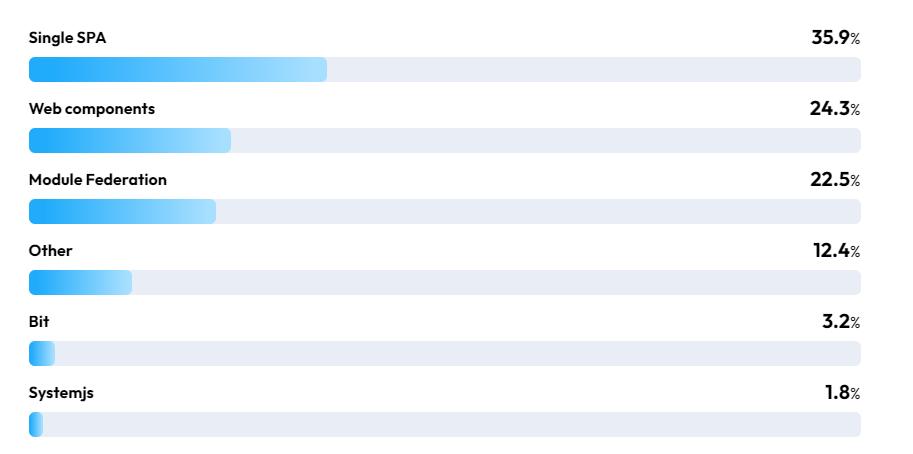
\includegraphics[width=\textwidth]{frontend_implementations_by_percent.png}
	\caption[Wykres procentowy popularności rozwiązań dla implementacji mikrofrontendów w 2022 roku]{Wykres procentowy popularności rozwiązań \\ dla implementacji mikrofrontendów w 2022 roku (źródło: \cite{tsh_2022})}
	\label{fig:tsh_frontend_implementations}
\end{figure}

Dla każdego z nich istnieje zestaw zastosowań biznesowych, dla których rozwiązanie nie będzie właściwe, ale będą istnieć też takie, dla których będą one właściwe. Każde z nich zostanie dokładniej omówione w poniższych podsekcjach.

\subsection{Konfiguracja serwera używająca routingu}
Konfigurowanie projektu, aby podawał do przeglądarki kod konkretnego mikrofrontendu w zależności od adresu URL można w prosty sposób wykonać poprzez odpowiednią konfigurację serwera. Taki sposób konfiguracji mkrofrontendów zalicza się do rozwiązań integrujących mikrofrontendy w czasie budowania projektu. To rozwiązanie jest wspierane przez najpopularniejsze oprogramowanie serwerowe takie jak IIS, Apache, NGINX. Konfiguracja serwera działa w bardzo prosty sposób - mapuje adresy URL na nazwy plików istniejących na serwerze oraz w zależności od tego, jaki aktualnie jest adres URL, przypisuje do zmiennej odpowiedni plik HTML. Odnosząc się do przykładu na listingu \cref{lst:nginx_microfrontends} (przykład pochodzi z \cite{fowler_2019}), taką zmienną jest \lstinline{$PAGE} z linii nr 8.

\lstinputlisting[style=htmlcssjs, label=lst:nginx_microfrontends, caption=Przykładowa implementacja mikrofrontendu wspomaganego przez nginx]{listings/nginx_microfrontends.html}

\subsection{Elementy <iframe>}
Najprostszym rozwiązaniem, obecnym już od dawna w standardzie języka znaczników HTML, jest element \lstinline{<iframe>}. Zgodnie z teorią, takie rozwiązanie spełnia założenia mikrofrontendów. Elementy \lstinline{<iframe>} wygodny sposób izolują poszczególne mikrofrontendy od siebie, nie pozwalają na nadpisanie się selektorów CSS oraz ewentualnych zmiennych globalnych w skrpytach JavaScript. Dzieje się tak ze względu na to, że elementy \lstinline{<iframe>} posiadają swój osobny zakres dla styli CSS i kodu JavaScript. Mimo to mają one też kilka wad. Po pierwsze, pełna izolacja kontekstu w elemencie \lstinline{<iframe>} powoduje, że treść tego elementu strony nie będzie reagowała na zmiany w~routingu. Ponadto, operowanie na historii przeglądania, adresie URL jest znacznie utrudnione. Taki koncept sprawia też trudności w przypadku, gdy znaczenie ma responsywność strony. Przykładowa implementacja, pochodząca z \cite{fowler_2019} znajduje się na listingu \cref{lst:iframe_microfrontends}

\lstinputlisting[style=htmlcssjs, label=lst:iframe_microfrontends, caption=Przykładowa implementacja mikrofrontendu za pomocą \lstinline{<iframe>}]{listings/iframe_microfrontends.html}

\subsection{Przechowywanie mikrofrontendów w skryptach JavaScript}
Idea ładowania mikrofrontendów przez podpinanie skryptów JavaScript jest bardzo prosta. Zgodnie z przykładem implementacji podanym na listingu \cref{lst:js_microfrontends} (przykład pochodzi z \cite{fowler_2019}), na początku sekcji \lstinline{<body>} podpiete są trzy skrypty reprezentujące trzy mikrofrontendy. Obecny jest także element \lstinline{<div id="micro-frontend-root">}, do którego będą ładowane mikrofrontendy. W skrypcie podanym niżej znajduje się przyporządkowanie tras w routingu do mikrofrontendów o odpowiednich nazwach oraz referencja na element \lstinline{<div id="micro-frontend-root">}.

\lstinputlisting[style=htmlcssjs, label=lst:js_microfrontends, caption=Przykładowa implementacja mikrofrontendu za pomocą JavaScript]{listings/microfrontends.html}

\subsection{Dynamiczne ładowanie modułów poprzez menedżer pakietów}
Istnieje również grupa rozwiązań oparta na dynamicznym ładowaniu modułów. Do grupy rozwiązań tego typu należą wspomniane na wykresie procentowym z  \cref{fig:tsh_frontend_implementations}, Module Federation, Bit oraz Systemjs. Pierwsze z rozwiązań, Module Federation, jest wtyczką do transpilatora Webpack. Wszystkie trzy, pomimo pewnych niewielkich różnic w~zakresie składni poleceń, instalacji i procesu konfiguracji, działają bardzo podobnie.

\subsection{Single SPA}
Single SPA jest frameworkiem, za pomocą którego można zrealizować koncepcję mikrofrontendów. Ten framework czerpie swój sposób działania z rozwiązań opartych na dynamicznym ładowaniu modułów. Jednocześnie pod skórą, ten framework stosuje wspomniany wcześniej Systemjs do samego przygotowania modułów, które są później dynaminicznie ładowane do treści strony. Istnieje też więc możliwość używania Single SPA z~każdym innym popularnym frameworkiem stosowanym przez programistów frontendu. Innowacją, którą proponuje Single SPA są predefiniowane konfiguracje, które automatyzują tworzenie mikrofrontedów. Do celów automatyzacji ustawiania infrastruktury mikrofrontendów twórcy udostępniają narzędzie CLI o nazwie \textit{create-single-spa}. Single SPA narzuca też sam z siebie określony podział konkrentych mikrofrontendów ze względu na zastosowania. Składnikami tego podziału są:

\begin{itemize}
	\item \textit{root-config} - mikrofrontend mający zastosowanie głównie przy agregacji innych mikrofrontendów,
	\item \textit{application} - domyślny typ mikrofrontendu bez specjalnych zadań projektowych,
	\item \textit{parcel} - reużywalny komponent, który jest niezależny w konstrukcji od frameworków używanych w projekcie; w przypadku użycia tylko jednego frameworka w całym projekcie, twórcy rekomendują \cite{singlespa-parcels} poleganie na systemie komponentyzacji tego frameworka.
\end{itemize}

Oprócz wymienionych możliwości, framework Single SPA udostępnia swój interfejs do testów jednostkowych i testów E2E oraz wspiera renderowanie kodu strony po stronie serwera. Dokumentacja frameworka Single SPA zawiera bardzo dokładne instrukcje postawienia środowiska oraz wdrożenia produkcyjnego pod każdy z popularnych frameworków, co znacząco obniża próg wejścia w samą koncepcję mikrofrontendów.

\chapter{Funkcjonalność badanej aplikacji}
Na potrzeby porównania obu architektur stworzona została aplikacja do zarządzania finansami osobistymi o roboczej nazwie Midas. W założeniu odbiorcami aplikacji mają być pojedyncze osoby lub gospodarstwa domowe, które chcą zadbać o kontrolę nad swoim budżetem domowym. Głównymi funkcjonalnościami aplikacji są:

\begin{itemize}
	\item możliwość wykonywania operacji CRUD w zakresie informacji o wydatkach i~przychodach poszczególnych użytkowników,
	\item system autoryzacji i uwierzytelniania spełniający aktualne normy w zakresie bezpieczeństwa aplikacji sieciowych,
	\item system uprawnień w obrębie rodziny (przykładowo użytkownik o roli rodzica może edytować transakcje na kontach dzieci, a dzieci nie mogą podglądać transakcji rodziców),
	\item przechowywanie paragonów i faktur w wersji elektronicznej i możliwość przypisania ich do konkretnej transakcji.
\end{itemize}

Podany zestaw funkcjonalności umożliwi wydzielenie kilku mikroserwisów, co zapewni wystarczającą bazę do symulowania połączeń między serwisami. Wykonanie jej w~architekturze ściśle mikroserwisowej pozwoli jednocześnie dobudować do tych mikroserwisów poszczególne mikrofrontendy tak, aby stanowiły one razem pełnoprawne aplikacje komunikujące się między sobą. Z drugiej strony pozwoli to też dobudować monolityczny frontend, który będzie komunikował się ze wszystkimi serwisami. Dzięki takiemu posunięciu, dla obu badanych projektów - monolitycznego oraz mikrofrotendowego, zapewnione będą jednolite warunki w zakresie komunikacji z~backendem, co będzie stanowiło bazę do porównania obu koncepcji architektonicznych w~zakresie wydajności i dostępności.

\chapter{Opis backendu projektu}
\section{Dobór technologii do projektu}
Do zrealizowania tej części projektu został wykorzystany język C\# oraz środowisko .NET. Użyto środowiska .NET w wersji 6.0, która jest jednocześnie najnowszą dostępną wersją LTS (\textit{Long Term Support}). Wspomniane technologie są dobrym wyborem do realizacji mikroserwisów ze względu na:

\begin{itemize}
	\item użycie paradygmatu programowania obiektowego i będący jego częścią polimorfizm, który sprzyja replikacji pojedynczego wzorca mikroserwisu,
	\item będący częścią środowiska .NET framework ASP.NET realizujący architekturę REST przy niewielkim narzucie w ilości kodu,
	\item istnienie wielu gotowych klas i modeli realizujących podstawowe funkcje sieciowe, takie jak autoryzacja i autentykacja, komunikacja z bazą za pomocą Entity Framework,
	\item generator NSwag służący do generowania klas w językach C\# oraz TypeScript reprezentujących metody kontrolerów poszczególnych mikroserwisów wykonanych w ASP.NET.
\end{itemize}

Środowiska mikroserwisowe są de facto oddzielnymi serwisami działającymi jednocześnie i pobierającymi dostępne zasoby. Do celów testów lokalnych na komputerze programisty zachodzi więc potrzeba zastosowania rozwiązania, które zminimalizuje użycie zasobów komputera tak, aby jednocześnie zachować wierność odwzorowania środowiska z wieloma serwerami. W celu osiągnięcia takiego efektu, zostało użyte oprogramowanie Docker służące do konteneryzacji środowisk. Za jego pomocą, używając specjalnych plików nazywanych obrazami, można tworzyć kontenery, którym Docker przydziela zasoby w czasie rzeczywistym tak, aby zoptymalizować ich użycie.
Razem z~narzędziem Docker, użyto też narzędzia \textit{docker-compose}, które umożliwia uruchomienie wielu kontenerów Dockera za pomocą pojedynczego skryptu.

Opisane technologie mogą też być komfortowo używane w połączeniu z~oprogramowaniem Docker służącym do konteneryzacji. Producent środowiska .NET, Microsoft udostępnił w serwisie Docker Hub obraz środowiska .NET z ustawionym frameworkiem ASP.NET oraz połączeniem z bazą SQL Server. Pozwala to na skorzystanie z gotowego środowiska, które jest konfigurowalne za pomocą pliku Dockerfile.

\section{Szablony projektów}
W celu zapewnienia skalowalności oraz łatwego tworzenia nowych serwisów, na potrzeby projektu opracowano dwa szablony projektu - zawierający wstępną autentykację użytkownika poprzez sprawdzanie zawartości nagłówka HTTP oraz taki, który jej nie zawiera.

Najważniejszą cechą tych szablonów jest możliwość szybkiego ustawienia nowego rozwiązania Visual Studio zawierającego ustawienia dla testów jednostkowych i~integracyjnych aplikacji, ustawienia plików \textit{Dockerfile} i \textit{docker-compose.yml} oraz ściśle określonego rozłożenia projektów w rozwiązaniu. Zapewnia to spójność kodu w zakresie całej aplikacji. W przypadku, gdyby nad kodem pojedynczego serwisu pracowało kilku programistów, mają oni ściśle narzuconą przez szablon strukturę kodu i podstawowa jego struktura zostanie zachowana. To z kolei powoduje, że wynikowo mimo tego, że nad poszczególnymi serwisami pracują różne osoby, ich struktura jest w dużym stopniu podobna. Ma to wiele zalet w zakresie zarządzania projektami, przykładowo:

\begin{itemize}
	\item pozwala na szybszą aklimatyzację programistów przenoszonych między projektami, bądź takich, których rola w zespole pomaga na wsparciu istniejących projektów,
	\item przyspiesza czas tworzenia nowych funkcjonalności oprogramowania,
	\item czas poświęcany na odtwórcze powtarzanie realizacji wzorca można poświęcić na ważniejsze czynności, takie jak redukcja długu technologicznego, zwiększanie pokrycia testami, itd.
\end{itemize}

\section{Podział backendu na serwisy}
Logika backendowa aplikacji została podzielona według funkcjonalności na serwisy opisane w poniższych podsekcjach.

\subsection{Hosting plików - File Storage Service}
Serwis z hostingiem plików odpowiada za przechowywanie wszystkich plików przekazanych aplikacji przez użytkownika. Są to między innymi zdjęcia profilowe użytkowników oraz pliki z dowodami wykonania transakcji przypisanych do konkretnych transakcji w ramach logiki domenowej. Serwis hostingu plików pozwala też na pobranie samego pliku o znanym identyfikatorze UUID oraz pobranie informacji o umieszczeniu pliku oraz konkretnych pobrań pliku.

\subsection{Autoryzacja - Authorization Service}
Serwis odpowiada za autoryzację użytkowników oraz operacje związane z~użytkownikami, które wymagają zachowania ostrożności pod kątem bezpieczeństwa aplikacji - tworzenie konta, logowanie do konta w aplikacji Midas, zmiana hasła. W tym serwisie przy logowaniu powstaje token JWT, który zapisany w ciasteczkach krąży po innych serwisach przekazywany przez nagłówek \textit{Authorization} w zapytaniu HTTP.

\subsection{Zarządzanie użytkownikami - User Service}
Serwis odpowiada za przechowywanie oraz umożliwienie dostępu do informacji o~użytkownikach. Obsługuje on też logikę związaną z kontami użytkowników, które nie wymagają zachowania szczególnej ostrożności w zakresie bezpieczeństwa aplikacji. Przykładem takiej operacji może być zmiana zdjęcia profilowego użytkownika.

\subsection{Zarządzanie rodzinami - Family Service}
Serwis odpowiada za przypisanie użytkowników do rodzin, których są członkami. Odpowiada też częściowo za uwierzytelnianie użytkownika - z tego serwisu pochodzą dane na temat tego, czy dany użytkownik ma wystarczające uprawnienia do edytowania danych dla swojej rodziny (ze względu na rolę przypisaną w systemie).

\subsection{Logika domenowa - Transaction Service}
Serwis ma za zadanie realizację operacji CRUD na transakcjach finansowych. Takimi operacjami może być wpisanie nowego wydatku do listy, usunięcie go z listy, pobranie listy wydatków w zależności do konkretnych parametrów (np. kategoria, czas, osoba z rodziny), dodanie pliku z dowodem wykonania transakcji.

\chapter{Opis badanych frontendów}
\section{Dobór technologii do projektów}
Do realizacji mikrofrontendów użyto biblioteki \textit{Single SPA}. Wspiera ona wszystkie najpopularniejsze frameworki do tworzenia aplikacji frontendowych. W badanych projektach użyto frameworka Angular ze względu na to, że najlepiej nadaje się do tworzenia dużych skalowalnych aplikacji. Ta cecha pozwoli utrzymać w ryzach potencjalnie rozwlekłą strukturę monolitycznej wersji projektu. W celu zapewnienia jak najmniejszych różnic technologicznych w projektach o różnej architekturze, wersja mikrofrontendowa będzie również używać frameworka Angular.

Do komunikacji z serwisami backendowymi, dla obu projektów użyto klas serwisów wygenerowanych przez generator NSwag. Będzie to działało tak, jak w przypadku klas w~języku C\# generowanych na potrzeby komunikacji między serwisami backendowymi. Różnica będzie tu jedynie taka, że te klasy będą gotowymi klasami w języku TypeScript dostosowanymi do użycia we frameworku Angular.

Ze względu na to, że walory estetyczne nie są istotne w zakresie rozważań nad mikrofrontendami, użyto gotowej biblioteki z elementami wizualnymi o nazwie \textit{angular-material}.

\section{Wersja monolityczna}
\section{Wersja mikroserwisowa}

\chapter{Porównanie projektów frontendowych}
\section{Wersjonowanie kodu}
\section{Wydajność}
\section{Dostępność}
\section{Testowanie kodu}
\section{Zależności między modułami i projektami}
\section{Możliwości w zakresie zarządzania projektami}
\section{Skalowalność}
\section{Koszty ustawienia środowiska produkcyjnego}

\chapter{Podsumowanie}

\printbibliography[heading=bibnumbered,title={Bibliografia}]

%\listoffigures

%\begingroup
%  \let\oldnumberline\numberline
%  \renewcommand{\numberline}[1]{Kod \oldnumberline{#1}}
%  \lstlistoflistings
%\endgroup

\beforelastpage

\end{document}
